%+++++++++++++++++++++++++++++++++++++++++++++++++++++++++++++++++++++++++++++++
%+++++++++++++++++++++++++++++++++++++++++++++++++++++++++++++++++++++++++++++++

%\mysubsection{Tutorial}

This section will show:
\bi
  \item A basic tutorial for a 1D mass and spring-damper with initial displacements, shortest possible model with practically no special settings
	\item A more advanced 2D rigid-body model ({\it coming soon})
	\item Links to examples section
\ei
%
The python source code of this section can be found in the file:
\bi
	\item[] \texttt{main/pythonDev/Examples/springDamperTutorial.py}
\ei
A large number of examples, some of them quite advanced, can be found in:
\bi
	\item[] \texttt{main/pythonDev/Examples}
	\item[] \texttt{main/pythonDev/TestModels}
\ei
This tutorial will set up a mass point and a spring damper, dynamically compute the solution and evaluate the reference solution.
\vspace{6pt}\\
%To start up, we set the system path to the directory of the library (needs to be adjusted; can be relative or absolute path):
%\pythonstyle
%\begin{lstlisting}[language=Python, firstnumber=1]
  %import sys 
  %sys.path.append('../../bin/WorkingRelease') #chose path of WorkingRelease!!!
%\end{lstlisting}
%
We import the exudyn library and the interface for all nodes, objects, markers, loads and sensors:
\pythonstyle
\begin{lstlisting}[language=Python, firstnumber=3]
  import exudyn as exu
  from exudyn.itemInterface import *
  import numpy as np #for postprocessing
\end{lstlisting}
%
Next, we need a SystemContainer, which contains all computable systems and add a new system.
Per default, you always should name your system 'mbs' (multibody system), in order to copy/paste code parts from other examples, tutorials and other projects:
\begin{lstlisting}[language=Python, firstnumber=6]
  SC = exu.SystemContainer()
  mbs = SC.AddSystem()
\end{lstlisting}
%
In order to check, which version you are using, you can printout the current \codeName\ version. This version is in line with the issue tracker and marks the number of open/closed issues added to \codeName :
\begin{lstlisting}[language=Python, firstnumber=8]
  print('EXUDYN version='+exu.__version__)
\end{lstlisting}
%
Using the powerful Python language, we can define some variables for our problem, which will also be used for the analytical solution:
\begin{lstlisting}[language=Python, firstnumber=9]
  L=0.5               #reference position of mass
  mass = 1.6          #mass in kg
  spring = 4000       #stiffness of spring-damper in N/m
  damper = 8          #damping constant in N/(m/s)
  f =80               #force on mass
\end{lstlisting}
%
For the simple spring-mass-damper system, we need initial displacements and velocities:
\begin{lstlisting}[language=Python, firstnumber=14]
  u0=-0.08            #initial displacement
  v0=1                #initial velocity
  x0=f/spring         #static displacement
  print('resonance frequency = '+str(np.sqrt(spring/mass)))
  print('static displacement = '+str(x0))
\end{lstlisting}
%
We first need to add nodes, which provide the coordinates (and the degrees of freedom) to the system.
The following line adds a 3D node for 3D mass point\footnote{Note: Point is an abbreviation for NodePoint, defined in \texttt{itemInterface.py}.}:
\begin{lstlisting}[language=Python, firstnumber=19]
  n1=mbs.AddNode(Point(referenceCoordinates = [L,0,0], 
                       initialCoordinates = [u0,0,0], 
                       initialVelocities = [v0,0,0]))
\end{lstlisting}
Here, \texttt{Point} (=\texttt{NodePoint}) is a Python class, which takes a number of arguments defined in the reference manual. The arguments here are \texttt{referenceCoordinates}, which are the coordinates for which the system is defined. The initial configuration is given by \texttt{referenceCoordinates + initialCoordinates}, while the initial state additionally gets \texttt{initialVelocities}.
The command \texttt{mbs.AddNode(...)} returns a \texttt{NodeIndex n1}, which basically contains an integer, which can only be used as node number. This node number will be used lateron to use the node in the object or in the marker.

%
While \texttt{Point} adds 3 unknown coordinates to the system, which need to be solved, we also can add ground nodes, which can be used similar to nodes, but they do not have unknown coordinates -- and therefore also have no initial displacements or velocities. The advantage of ground nodes (and ground bodies) is that no constraints are needed to fix these nodes.
%
Such a ground node is added via:
\begin{lstlisting}[language=Python, firstnumber=22]
  nGround=mbs.AddNode(NodePointGround(referenceCoordinates = [0,0,0]))
\end{lstlisting}
%
In the next step, we add an object\footnote{For the moment, we just need to know that objects either depend on one or more nodes, which are usually bodies and finite elements, or they can be connectors, which connect (the coordinates of) objects via markers, see Section \ref{sec:programStructure}.}, which provides equations for coordinates. The \texttt{MassPoint} needs at least a mass (kg) and a node number to which the mass point is attached. Additionally, graphical objects could be attached:
\begin{lstlisting}[language=Python, firstnumber=23]
  massPoint = mbs.AddObject(MassPoint(physicsMass = mass, nodeNumber = n1))
\end{lstlisting}
%
In order to apply constraints and loads, we need markers. These markers are used as local positions (and frames), where we can attach a constraint lateron. In this example, we work on the coordinate level, both for forces as well as for constraints.
Markers are attached to the according ground and regular node number, additionally using a coordinate number (0 ... first coordinate):
\begin{lstlisting}[language=Python, firstnumber=24]
  groundMarker=mbs.AddMarker(MarkerNodeCoordinate(nodeNumber= nGround, 
                                                  coordinate = 0))
  #marker for springDamper for first (x-)coordinate:
  nodeMarker = mbs.AddMarker(MarkerNodeCoordinate(nodeNumber= n1, 
                                                  coordinate = 0))
\end{lstlisting}
This means that loads can be applied to the first coordinate of node \texttt{n1} via marker with number \texttt{nodeMarker},
which is in fact of type \texttt{MarkerIndex}.

Now we add a spring-damper to the markers with numbers \texttt{groundMarker} and the \texttt{nodeMarker}, providing stiffness and damping parameters:
\begin{lstlisting}[language=Python, firstnumber=29]
  mbs.AddObject(CoordinateSpringDamper(markerNumbers = [groundMarker, nodeMarker], 
                                       stiffness = spring, 
                                       damping = damper)) 
\end{lstlisting}
%
A load is added to marker \texttt{nodeMarker}, with a scalar load with value \texttt{f}:
\begin{lstlisting}[language=Python, firstnumber=32]
  nLoad = mbs.AddLoad(LoadCoordinate(markerNumber = nodeMarker, 
                                     load = f))
\end{lstlisting}
%
Finally, a sensor is added to the coordinate constraint object \texttt{nC}, requesting the outputvariable \texttt{Force}:
\begin{lstlisting}[language=Python, firstnumber=34]
  mbs.AddSensor(SensorObject(objectNumber=nC, fileName='groundForce.txt', 
                             outputVariableType=exu.OutputVariableType.Force))
\end{lstlisting}
Note that sensors can be attached, e.g., to nodes, bodies, objects (constraints) or loads.
%
As our system is fully set, we can print the overall information and assemble the system to make it ready for simulation:
\begin{lstlisting}[language=Python, firstnumber=36]
  print(mbs)
  mbs.Assemble()
\end{lstlisting}
%
We will use time integration and therefore define a number of steps (fixed step size; must be provided) and the total time span for the simulation:
\begin{lstlisting}[language=Python, firstnumber=38]
  steps = 1000  #number of steps to show solution
  tEnd = 1     #end time of simulation
\end{lstlisting}
%
All settings for simulation, see according reference section, can be provided in a structure given from \texttt{exu.SimulationSettings()}. Note that this structure will contain all default values, and only non-default values need to be provided:
\begin{lstlisting}[language=Python, firstnumber=40]
  simulationSettings = exu.SimulationSettings()
  simulationSettings.solutionSettings.solutionWritePeriod = 5e-3  #output interval general
  simulationSettings.solutionSettings.sensorsWritePeriod = 5e-3  #output interval of sensors
  simulationSettings.timeIntegration.numberOfSteps = steps
  simulationSettings.timeIntegration.endTime = tEnd
\end{lstlisting}
%
We are using a generalized alpha solver, where numerical damping is needed for index 3 constraints. As we have only spring-dampers, we can set the spectral radius to 1, meaning no numerical damping:
\begin{lstlisting}[language=Python, firstnumber=45]
  simulationSettings.timeIntegration.generalizedAlpha.spectralRadius = 1
\end{lstlisting}
%
In order to visualize the results online, a renderer can be started. As our computation will be very fast, it is a good idea to wait for the user to press SPACE, before starting the simulation (uncomment second line):
\begin{lstlisting}[language=Python, firstnumber=46]
  exu.StartRenderer()              #start graphics visualization
  #mbs.WaitForUserToContinue()    #wait for pressing SPACE bar to continue
\end{lstlisting}
As the simulation is still very fast, we will not see the motion of our node. Using e.g.\ \texttt{steps=10000000} in the lines above allows you online visualize the resulting oscillations.

%
Finally, we start the solver, by telling which system to be solved, solver type and the simulation settings:
\begin{lstlisting}[language=Python, firstnumber=48]
  SC.TimeIntegrationSolve(mbs, 'GeneralizedAlpha', simulationSettings)
\end{lstlisting}
%

After simulation, our renderer needs to be stopped (otherwise it would stay in background and prohibit further simulations). 
Sometimes you would like to wait until closing the render window, using \texttt{WaitForRenderEngineStopFlag()}:
\begin{lstlisting}[language=Python, firstnumber=49]
  #SC.WaitForRenderEngineStopFlag()#wait for pressing 'Q' to quit
  exu.StopRenderer()               #safely close rendering window!
\end{lstlisting}
%
There are several ways to evaluate results, see the reference pages. In the following we take the final value of node \texttt{n1} and read its 3D position vector:
\begin{lstlisting}[language=Python, firstnumber=51]
  #evaluate final (=current) output values
  u = mbs.GetNodeOutput(n1, exu.OutputVariableType.Position)
  print('displacement=',u)
\end{lstlisting}
%
The following code generates a reference (exact) solution for our example:
\begin{lstlisting}[language=Python, firstnumber=54]
  import matplotlib.pyplot as plt
  import matplotlib.ticker as ticker

  omega0 = np.sqrt(spring/mass)  #eigen frequency of undamped system
  dRel = damper/(2*np.sqrt(spring*mass)) #dimensionless damping
  omega = omega0*np.sqrt(1-dRel**2) #eigen freq of damped system
  C1 = u0-x0 #static solution needs to be considered!
  C2 = (v0+omega0*dRel*C1) / omega #C1, C2 are coeffs for solution

  refSol = np.zeros((steps+1,2))
  for i in range(0,steps+1):
    t = tEnd*i/steps
    refSol[i,0] = t
    refSol[i,1] = np.exp(-omega0*dRel*t)*(C1*np.cos(omega*t)+C2*np.sin(omega*t))+x0

  plt.plot(refSol[:,0], refSol[:,1], 'r-', label='displacement (m); exact solution')
\end{lstlisting}
%
Now we can load our results from the default solution file \texttt{coordinatesSolution.txt}, which is in the same
directory as your python tutorial file. For convenient reading the file containing commented lines, we use a numpy feature and
finally plot the displacement of coordinate 0 or our mass point\footnote{\texttt{data[:,0]} contains the simulation time, \texttt{data[:,1]} contains displacement of (global) coordinate 0, \texttt{data[:,2]} contains displacement of (global) coordinate 1, ...)}:
\begin{lstlisting}[language=Python, firstnumber=73]
  data = np.loadtxt('coordinatesSolution.txt', comments='#', delimiter=',')
  plt.plot(data[:,0], data[:,1], 'b-', label='displacement (m); numerical solution') 
\end{lstlisting}
The sensor result can be loaded in the same way. The sensor output format contains time in the first column and sensor values in the remaining columns. The number of columns depends on the 
sensor and the output quantity (scalar, vector, ...):
\begin{lstlisting}[language=Python, firstnumber=75]
  data = np.loadtxt('groundForce.txt', comments='#', delimiter=',')
  plt.plot(data[:,0], data[:,1]*1e-3, 'g-', label='force (kN)')
\end{lstlisting}

%
In order to get a nice plot within Spyder, the following options can be used\footnote{note, in some environments you need finally the command \texttt{plt.show()}}:
\begin{lstlisting}[language=Python, firstnumber=77]
  ax=plt.gca() # get current axes
  ax.grid(True, 'major', 'both')
  ax.xaxis.set_major_locator(ticker.MaxNLocator(10))
  ax.yaxis.set_major_locator(ticker.MaxNLocator(10))
  plt.legend() #show labels as legend
  plt.tight_layout()
  plt.show() 
\end{lstlisting}
%

The matplotlib output should look like this:
\begin{center}
  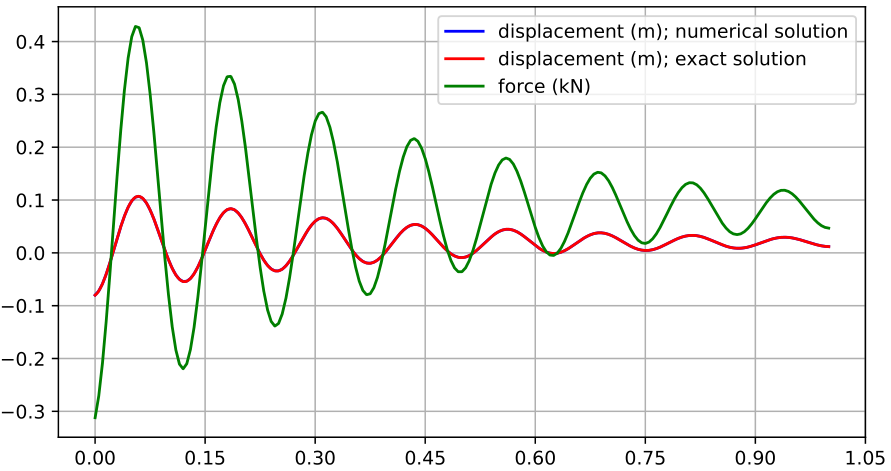
\includegraphics[height=6cm]{../demo/screenshots/plotSpringDamper}
\end{center}
%
\vspace{24pt}
Further examples can be found in your copy of exudyn: 
\bi
  \item[] \texttt{main/pythonDev/Examples}
  \item[] \texttt{main/pythonDev/TestModels}
\ei


